\documentclass[a4paper,12pt]{article} 
\usepackage{apacite}
\usepackage{natbib}
\usepackage{geometry}
\usepackage{ctex} 
\usepackage{setspace}
\usepackage{enumerate}
\usepackage{amsmath}
\usepackage{subfigure}
\usepackage{caption}
\usepackage{listings}
\usepackage{ctex}

% 用来设置附录中代码的样式

\lstset{
	basicstyle          =   \sffamily,          % 基本代码风格
	keywordstyle        =   \bfseries,          % 关键字风格
	commentstyle        =   \rmfamily\itshape,  % 注释的风格,斜体
	stringstyle         =   \ttfamily,  % 字符串风格
	flexiblecolumns,                % 别问为什么,加上这个
	numbers             =   left,   % 行号的位置在左边
	showspaces          =   false,  % 是否显示空格,显示了有点乱,所以不现实了
	numberstyle         =   \zihao{-5}\ttfamily,    % 行号的样式,小五号,tt等宽字体
	showstringspaces    =   false,
	captionpos          =   t,      % 这段代码的名字所呈现的位置,t指的是top上面
	frame               =   lrtb,   % 显示边框
}

\lstdefinestyle{Python}{
	language        =   Python, % 语言选Python
	basicstyle      =   \zihao{-5}\ttfamily,
	numberstyle     =   \zihao{-5}\ttfamily,
	keywordstyle    =   \color{blue},
	keywordstyle    =   [2] \color{teal},
	stringstyle     =   \color{magenta},
	commentstyle    =   \color{red}\ttfamily,
	breaklines      =   true,   % 自动换行,建议不要写太长的行
	columns         =   fixed,  % 如果不加这一句,字间距就不固定,很丑,必须加
	basewidth       =   0.5em,
}
\setstretch{1.4} 
\bibliographystyle{unsrt}
\usepackage{graphicx}
\geometry{a4paper,left=2.5cm,right=2.5cm,top=2cm,bottom=2cm}
\title{\bfseries 基于快速傅里叶变换和角谱理论的衍射仿真}
\author{\normalsize 少年班学院\quad PB22000251\quad 张鸣轩 \\ \normalsize 物理学院\quad PB22020603 \quad 涂婳}
\date{\small 2024年1月1日}
\begin{document}
	\maketitle
	\begin{abstract}
		 	本文以光学中的菲涅尔衍射为主题,基于快速傅里叶变换使用Python模拟衍射现象,得到了给定衍射屏的像。再通过角谱理论,分析了自由光场下光的传播模拟,探究了矩孔衍射的两种模拟实现。
	\end{abstract}
	\begin{center}
		\textbf{\bfseries 关键词:} 【快速傅里叶变换 】,【菲涅尔衍射】,【角谱理论】
	\end{center}
	
	\tableofcontents
	\newpage
	\section{背景介绍}
	
		菲涅尔在1815年与1818年进行了光的波动性的计算,并构想了光以球面波连续不断的传播出去。随后在对光的波动性的认识更加深刻后,得到了菲涅尔-基尔霍夫衍射公式。随着现代计算科学的发展,对于傅里叶变换这一信号分析方法,得到了离散傅里叶变换的计算方法。在计算菲涅尔衍射中,离散傅里叶变换的近似模拟可以很好的解决衍射问题。
	\section{原理介绍}
	\subsection{离散傅里叶变换}
	通过傅里叶变换,我们可以将时域上的函数变换为频域上的函数:
	$$F(f)=\int_{-\infty}^{+\infty}f(t)e^{-j2\pi ft}dt$$
	因为计算机采集的信号在时域中式离散的,所以实际应用中函数为离散的函数$f_s(t)$,相对应的频域上的函数$F_s(t)$也是离散的。通过采样和时域离散化等近似,可以得到频域离散化的计算结果。设离散信号的表达式为:
	$$x_s(t)=\sum_{n=0}^{N-1}x(t)\delta(t-nT_s)$$
	离散信号的傅里叶级数:
	$$X(k\omega_{0})=\frac{1}{T_{0}}\int_{0}^{T}(\sum_{n=0}^{N-1}x(t)\delta(t-nT_{s}))e^{-jkw_{0}t}dt$$
	利用狄拉克函数的性质,得到离散的频域函数:
	$$X[k]=\frac1N\sum_{n=0}^{N-1}x[n]e^{-j\frac{2\pi}Nkn}$$	
	\begin{center}其中$x[n]=x(nT_s)$,$X[k]=X(k\omega_0)T_s$\end{center}
		\begin{center}
	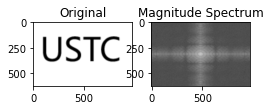
\includegraphics[scale=0.75]{Pic1.png}\\
	图1.离散傅里叶变换示意图
	\end{center}\vspace{0.2cm}
	
	
\newpage
	\subsection{利用DFT与菲涅尔衍射积分的同构性模拟衍射}
\noindent 对于光波在空间中的自由传播,如何由已知平面上的光波复振幅分布,来获知后续空间中任意位置的光波复振幅,是光学的基本问题之一。

\noindent 为此,我们构建以下情境:一束光线穿过一个孔径为$S'$的平面,在距离屏幕为d的时候,考虑在屏上的光场波函数。

\noindent 该波函数可以由菲涅尔积分定义:
$$\Psi(\pmb r,t)=C\int_{S'}\frac{e^{ik|r-r'|}}{|r-r'|}cos(\theta)d^2r'$$
$$(C=\frac{k\Psi_0e^{-itw}}{2\pi i})$$
基于菲涅尔近似,在角度$\theta$接近0度时(傍轴条件下),上式存在简化:
$$
|r-r'|\approx z+\frac{(x-x')^2+(y-y')^2}{2z}
$$
此时,我们还可以假设$|r-r'|\approx d$
于是菲涅尔积分变成:
$$
\Psi(\pmb r,t)=R\int_{-\infty}^{+\infty}\int_{-\infty}^{+\infty}f(x',y')e^{\frac{ik}{2z}(x'^2+y'^2)}e^{-\frac{ikx}{z}x'-\frac{iky}{z}y'}dx'dy'
$$
其中:
$$
R=\frac{k\Psi_0e^{i(kz-tw)}}{2\pi iz}e^{ik\frac{x^2+y^2}{2z}}
$$

$$
f(x',y')=\begin{cases}
	1 ,\quad (x',y')\in S'\\
	0,\quad(x',y')\notin S'\\
\end{cases}
$$

\noindent 令$\mathcal F$为傅里叶变换,有计算公式:
$$
\mathcal F[f(x',y')e^{\frac{ik}{2z}(x'^2+y'^2)}]=\int_{-\infty}^{+\infty}\int_{-\infty}^{+\infty}f(x',y')e^{\frac{ik}{2z}(x'^2+y'^2)}e^{-\frac{ikx}{z}x'-\frac{iky}{z}y'}dx'dy'
$$
恰与菲涅尔积分表达式积分部分相同,

\noindent 从而上式可转换成傅里叶变换形式:
$$
\Psi(\pmb r,t)=R\cdot \mathcal F[f(x',y')e^{\frac{ik}{2z}(x'^2+y'^2)}]
$$
综上,我们可以利用傅里叶变换来直接求解衍射屏上光场的波函数。

\noindent 将以上内容写成复振幅形式,可得:
$$
U(x,y,d)=\frac{e^{ikd}}{i\lambda d}e^{ik\frac{x^2+y^2}{2d}}\int_{-\infty}^{+\infty}\int_{-\infty}^{+\infty}U(x',y',0)e^{\frac{ik}{2d}(x'^2+y'^2)}e^{-\frac{ikx}{d}x'-\frac{iky}{d}y'}dx'dy'
$$

$$
=\frac{e^{ikd}}{i\lambda d}e^{ik\frac{x^2+y^2}{2d}}\mathcal F[U(x',y')e^{\frac{ik}{2d}(x'^2+y'^2)}]
$$

\noindent 另外,在菲涅尔衍射近似的基础上,还可以利用夫琅禾费近似,对二次相位因子再进一步进行近似,方法如下:

\noindent 在菲涅尔衍射积分中,相位因子中存在x'与y‘(衍射屏上垂直方向的坐标)的二次项,若这一部分对相位的影响较小,即:
$$
z\ll\frac{k}{2}(x'^2+y'^2)_{max}
$$
此时可以忽略掉$e^{\frac{ik}{2z}(x'^2+y'^2)}$项的影响,从而得到夫琅禾费近似的结果:
$$
\Psi(\pmb r,t)=R\int_{-\infty}^{+\infty}\int_{-\infty}^{+\infty}f(x',y')e^{-\frac{ikx}{z}x'-\frac{iky}{z}y'}dx'dy'
$$

$$
R=\frac{k\Psi_0e^{i(kz-tw)}}{2\pi iz}e^{ik\frac{x^2+y^2}{2z}}
$$

\noindent 由于:
$$
\mathcal F[f(x',y')]=\int_{-\infty}^{+\infty}\int_{-\infty}^{+\infty}f(x',y')^{-\frac{ikx}{z}x'-\frac{iky}{z}y'}dx'dy'
$$
最终有:
$$
\Psi(\pmb r,t)=R\cdot \mathcal F[f(x',y')]
$$
写成复振幅形式,得:
$$
U(x,y,d)=\frac{e^{ikd}}{i\lambda d}e^{ik\frac{x^2+y^2}{2d}}\int_{-\infty}^{+\infty}\int_{-\infty}^{+\infty}U(x',y',0)e^{-\frac{ikx}{d}x'-\frac{iky}{d}y'}dx'dy'
$$

$$
=\frac{e^{ikd}}{i\lambda d}e^{ik\frac{x^2+y^2}{2d}}\mathcal F[U(x',y')]
$$

\noindent 虽然上述夫琅禾费近似条件较为苛刻,但在透镜系统中可以很好地实现,进一步简化了运算。
	\newpage
		
	\subsection{利用角谱传播理论从频谱角度模拟衍射}
	\begin{center}
	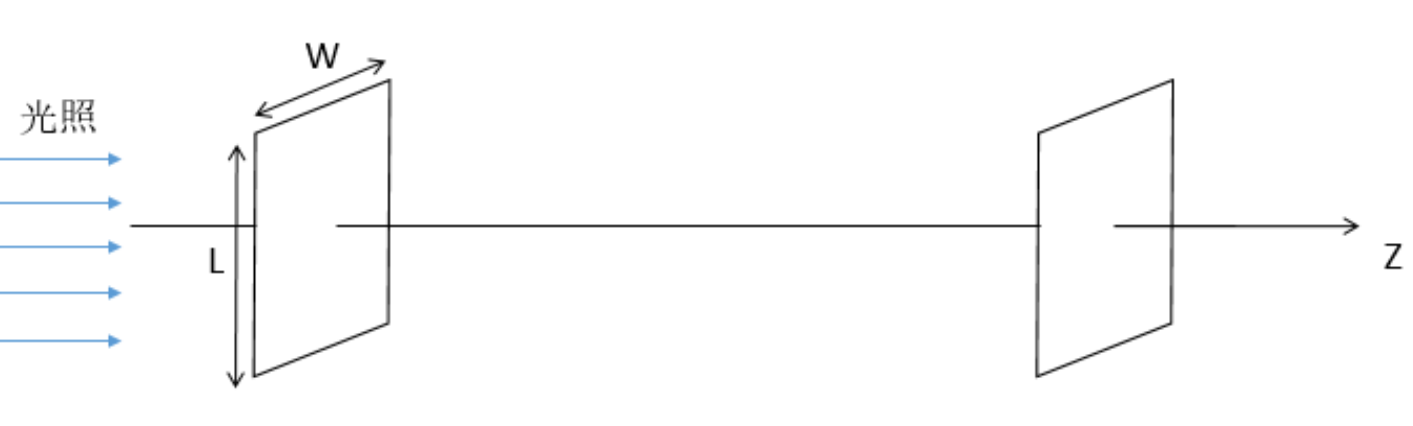
\includegraphics[scale=0.4]{Pica4.png}\\
	图2.衍射光传播示意图
\end{center}\vspace{0.2cm}\par
		傅里叶光学中,构建了角谱传播理论,即从频谱的角度来分析光的传播规律。
		
		其主要思路为,先对原光场进行傅里叶变换,得到其频谱后,结合亥姆霍兹方程,得到衍射位置光场的频谱,对其做傅里叶逆变换,即可得到衍射光场。
		
		情境构造:已知z=0的平面光波(复振幅)分布为$U(x,y,0)$,求解当光传播z距离之后的光波(复振幅)分布。
		
		\noindent 对原光场进行傅里叶变换:
		$$
		U(x,y,0)=\int_{-\infty}^{+\infty}\int_{-\infty}^{+\infty}A(f_x,f_y,0)e^{-i2\pi (f_xx+f_yy)}df_xdf_y
		$$
		其中$A(f_x,f_y,0)$表示在z=0平面上$U(x,y,0)$的频谱。
		
		\noindent 由于光是电磁波,且在自由空间中传播是无源的,故$U(x,y,0)$满足亥姆霍兹方程:
		$$
		\nabla^2 U+k^2U=0
		$$
		此二阶微分方程可以利用积分变换求解如下:
		
		\noindent 由于衍射平面与xy平面平行,故我们考虑将$U(x,y,0)$在xy平面上进行傅里叶变换。
		
		\noindent 为体现与频率的关系,我们采取傅里叶变换:$(x,y)\leftrightarrow(f_x,f_y)$
		$$
		\begin{cases}
			G(f)=\int^{+\infty}_{-\infty}g(x)e^{-i2\pi f_x}dx\\
			g(x)=\int^{+\infty}_{-\infty}G(x)e^{i2\pi f_x}df\\
		\end{cases}
		$$
		以及二维傅里叶变换:
		$$
		\begin{cases}
			G(f_x,f_y)=\int^{+\infty}_{-\infty}\int^{+\infty}_{-\infty}g(x,y)e^{-i2\pi (f_xx+f_yy)}dxdy\\
			g(x,y)=\int^{+\infty}_{-\infty}\int^{+\infty}_{-\infty}G(f_x,f_y)e^{i2\pi (f_xx+f_yy)}df_xdf_y\\
		\end{cases}
		$$
		对$\frac{\partial^2 U}{\partial x^2}+\frac{\partial^2 U}{\partial y^2}+\frac{\partial^2 U}{\partial z^2}+k^2U=0$进行二维傅里叶变换,得到:
		$$
		-4\pi^2(f_x^2+f_y^2)G_z+\frac{d^2 G_z}{d z^2}+k^2G_z=0
		$$
		其中$G_z(f_x,f_y,z)$是$U(x,y,z)$经xy二维傅里叶变换后的结果,亦即:
		$$
		\frac{d^2}{dz^2}G(f_x,f_y,z)+4\pi^2[\frac{1}{\lambda^2}-f_x^2-f_y^2]G(f_x,f_y,z)=0
		$$
		此二阶微分方程的一个基元解为:
		$$
		A(f_x,f_y,z)=A(f_x,f_y,0)e^{i2\pi z\sqrt{\frac{1}{\lambda^2}-f_x^2-f_y^2}}
		$$
		从而我们得到了衍射面的频谱与初始频谱之间的关系,具体来说,主要是在不同的频率分量上引入了相位偏移。
		
		\noindent 其中具有传播的限制条件:$f_x^2+f_y^2<\frac{1}{\lambda^2}$,即光无法传播空间 频率大于$\frac{1}{\lambda}$的频率。
		
		\noindent 对z距离下的频谱进行傅里叶逆变换:
		$$
		U(x,y,z)=\mathcal F^{-1}\{\mathcal F[U(x,y,0)]e^{i2\pi z\sqrt{\frac{1}{\lambda^2}-f_x^2-f_y^2}}\}
		$$
		即可得到传播z距离后的光场复振幅分布:
		$$
		U(x,y,z)=\int_{-\infty}^{+\infty}\int_{-\infty}^{+\infty}A(f_x,f_y,0)e^{i2\pi z\sqrt{\frac{1}{\lambda^2}-f_x^2-f_y^2}}circ(\frac{\sqrt{f_x^2+f_y^2}}{\lambda})e^{-i2\pi (f_xx+f_yy)}df_xdf_y
		$$
		该法未使用任何近似。
	
	\subsection{算法实现}
	\noindent\textbf{利用FFT变换图片到频域:\\}
本实验主要使用opencv.cv2库进行图像识别,使用numpy库中的np.fft.fft2()函数进行快速傅里叶变换,如图3,4,是采用了快速傅里叶变换后的频域函数图。
	\begin{center}
	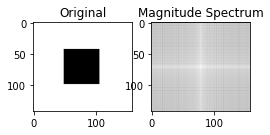
\includegraphics[scale=0.75]{Pica2.png}\\
	图3.离散傅里叶变换示意图
\end{center}\vspace{0.2cm}
	\begin{center}
	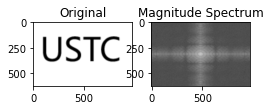
\includegraphics[scale=0.75]{Pic1.png}\\
	图4.离散傅里叶变换示意图
\end{center}\vspace{0.2cm}
	\begin{center}
	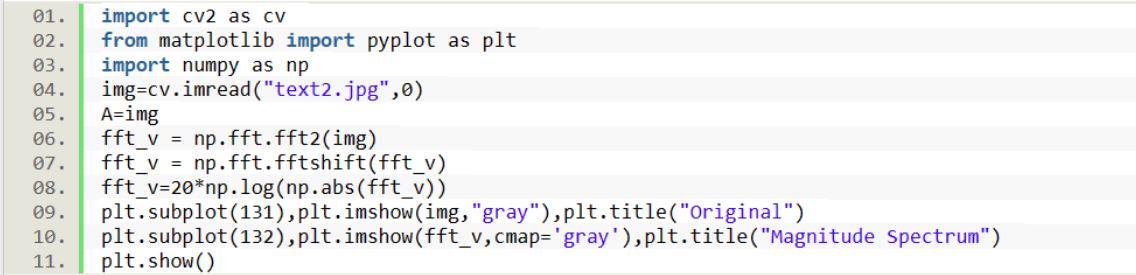
\includegraphics[scale=0.85]{Pica3.png}\\
	图5.代码实现
\end{center}\vspace{0.2cm}
\noindent\textbf{利用DFT与菲涅尔衍射积分的同构性模拟衍射:\\}
根据2.2节,菲涅尔衍射公式在近似后可表示为:
$$\mathrm{U(r,t)=R\cdot\mathcal{F}[f(x',y')e^{\frac{ik}{2z}(x'^2+y'^2)}]}$$
$$\mathcal{F}[\mathrm{f(x',y')e^{\frac{ik}{2z}(x'^2+y'^2)}}]=\int_{-\infty}^{\infty}\int_{-\infty}^{\infty}\mathrm{f(x',y')e^{\frac{ik}{2z}(x'^2+y'^2)}e^{-\frac{ikx}{z}x'-\frac{iky}{z}y'}dx'dy'}$$
np.fft.fft2()可以进行傅里叶变换,但只可以处理离散情况,所以要对衍射屏进行分割,并假设可通光处为同一相位,同一振幅,即复振幅$\widetilde{U}=1$。不可通光处,$\widetilde{U}=0$。\\
如果将图片的长宽像素设为$L_x$和$L_y$,将他们划为等间距的$N_x$和$N_y$份,衍射屏的坐标可以表示为:
$$\mathrm x'_\mathrm{n_x}=\left\{-\mathrm L_\mathrm{x}+\mathrm n_\mathrm{x}\dfrac{2\mathrm L_\mathrm{x}}{\mathrm N_\mathrm{x}},\quad0\le\mathrm n_\mathrm{x}\le\mathrm N_\mathrm{x}-1\right\}$$
$$\mathrm y'_\mathrm{n_y}=\left\{-\mathrm L_\mathrm{y}+\mathrm n_\mathrm{y}\dfrac{2\mathrm L_\mathrm{y}}{\mathrm N_\mathrm{y}},\quad0\le\mathrm n_\mathrm{y}\le\mathrm N_\mathrm{y}-1\right\}$$
离散傅里叶变换表示为:
$$\mathrm{\mathcal{F}(u_x,u_y)=\sum_{n_x=0}^{N_x-1}\sum_{n_y=0}^{N_y-1}U(x_{n_x}^{\prime},y_{n_y}^{\prime})e^{-i2\pi u_x\frac{n_x}{N_x}-i2\pi u_y\frac{n_y}{N_y}}}$$
最后只需要乘$R(r,t)$就可以得到最后像的复振幅。
\newpage 具体算法实现如下:
\begin{enumerate}[I.]
	\item 设置参数,读入图片,通过像素数量计算分割为$N_x$和$N_y$份,计算出相应的坐标值。
	\item 计算出函数$f(x',y')=U(x',y')e^{\frac{ik}{2z}(x'^2+y'^2)}$,对其进行快速傅里叶展开,得到$\mathcal{FFT}(f)$。
	\item 计算像屏上的函数$R(x,y)$,乘以$\mathcal{FFT}(f)$便得到像屏上的复振幅。
	\item 计算光强分布,输出图像。
\end{enumerate}
\begin{center}
	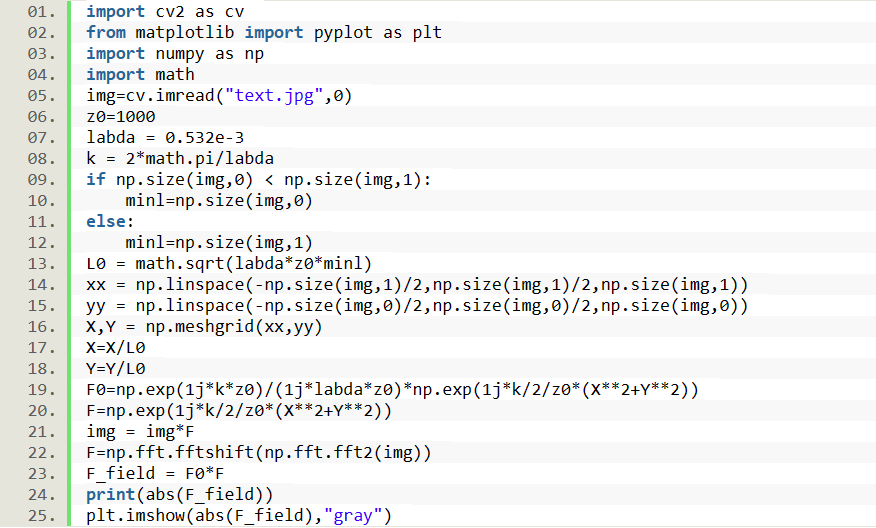
\includegraphics[scale=1.05]{Pica5.png}\\
	图6.代码实现
\end{center}\vspace{0.2cm}
\noindent\textbf{利用角谱传播理论从频谱角度模拟衍射:}\\
根据2.3节$U(x,y,z)=\mathcal F^{-1}\{\mathcal F[U(x,y,0)]e^{i2\pi z\sqrt{\frac{1}{\lambda^2}-f_x^2-f_y^2}}\}$,设计算法如下:
\begin{enumerate}
	\item 设置参数,读入图片,通过像素数量计算分割为$N_x$和$N_y$份,计算出相应的坐标值。
	\item 计算出函数$f(x',y')=U(x',y')$,对其进行快速傅里叶展开,得到$\mathcal{FFT}(f)$。
	\item 对频域函数进行判断,截断$f_x^2+f_y^2>\frac{1}{\lambda^2}$的部分。
	\item 新的频域函数乘$e^{i2\pi z\sqrt{\frac{1}{\lambda^2}-f_x^2-f_y^2}}$,再进行一次傅里叶逆变换便得到像屏上的复振幅。
	\item 计算光强分布,输出图像。
\end{enumerate}

\newpage	
\section{实验现象与数据处理}
	\subsection{同构性模拟衍射实验现象}
\begin{center}
	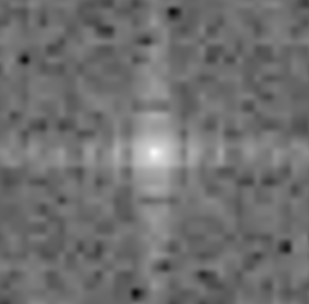
\includegraphics[scale=1.05]{Pica6.png}\\
	图7.矩孔衍射模拟
\end{center}\vspace{0.2cm}
如图七所示,是利用DFT与菲涅尔衍射积分的同构性模拟矩孔衍射,但图像噪点较多,且实验现象不明显,仅能大致看到因为衍射而产生的间断亮暗衍射图样。分析实验判断可能是离散傅里叶变换是对图像内有限点采样模拟,在频域上的傅里叶函数并不能实现准确而产生较大误差。
\subsection{角谱传播理论模拟衍射实验现象}
\begin{center}
	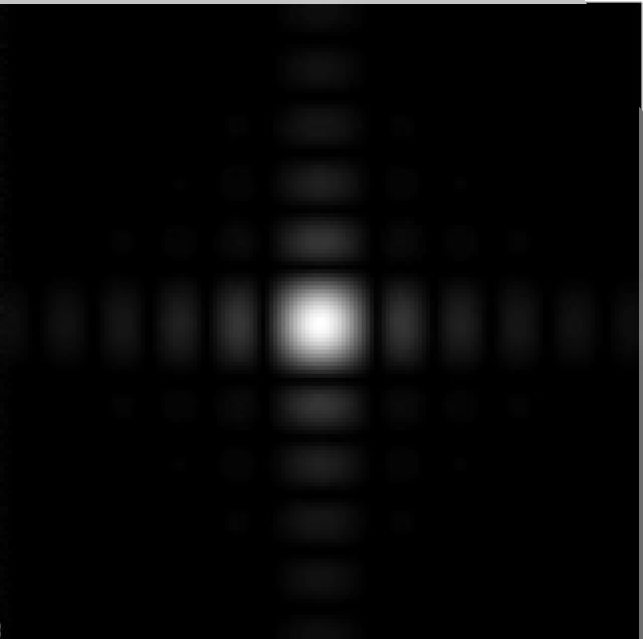
\includegraphics[scale=0.25]{Pica8.png}\\
	图8.矩孔衍射的角谱模拟
\end{center}\vspace{0.2cm}
如图八,是利用角谱传播理论从频谱角度模拟衍射,因为角谱理论采用了较小的近似,且对高频部分进行了截断,所以实验现象较好。
\newpage	

\section{展望}
	在本实验中,采用了快速傅里叶变换进行模拟,快速傅里叶变换在信号学,信息科学,计算机科学与固体物理等领域有较高应用价值,如密度泛函理论和图像识别都是其应用。其次,本实验还从矩孔衍射出发,探讨了多张不同图片的频谱展开,及利用其频谱展开进一步得到了衍射图样,是傅里叶光学的一种应用前景。
		
	\section{总结}
	\begin{enumerate}[I.]
\item 通过傅里叶变换,可以采用同构和角谱的方式来计算衍射,实验现象明显。
\item 通过快速傅里叶变换,可以得到给定图片的频域展开。
\item 矩孔衍射图像符合理论推导,出现了明暗相间的衍射图样。
\end{enumerate}
	\textbf{参考文献}\\ \relax
[1]《光学》 赵凯华,钟锡华\\ \relax
[2]Contemporary Optical Image Processing with MATLAB  ,Ting-Chung Poon\\ \relax
[3]Introduction to Computer Holography, Kyoji Matsushima, 2020\\ \relax
[4]Computational Fourier Optics a MATLAB tutorial (SPIE Tutorial Texts Vol. TT89)

	
\end{document}
